\documentclass[a4paper,10pt,titlepage]{article}
\usepackage{color}
\usepackage{wrapfig}
\usepackage[dvipdfm]{geometry}
\usepackage{amsmath}
\usepackage{amsfonts}
\usepackage[utf8]{inputenc}
\usepackage{amssymb}
\usepackage{graphicx}
\usepackage{fancyhdr}
\usepackage{svnkw}
\usepackage{tabularx}
\usepackage{ngerman}
\pagestyle{fancy}
\evensidemargin0mm
\oddsidemargin0mm
\setlength{\listparindent}{0pt}
\setlength{\parskip}{0pt}
\voffset-10mm
\topmargin0mm
\headsep10mm
\headheight20mm
\lhead{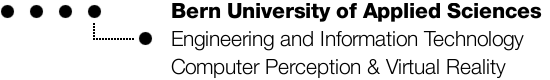
\includegraphics[width=40mm]{logo_ti.png}\newline}
\rhead{Stefan Heinemann (heins4)\\Christoph Isch (ischc2)}
\lfoot{\today}

\title{Documentation}
\author{heins4: Stefan Heinemann\\ischc2: Christoph Isch}
\begin{document}

\begin{titlepage}
{\huge Project Specifications}\\
\textbf{heins4: Stefan Heinemann}\\
\textbf{ischc2: Christoph Isch}\\
\newline\newline\newline\newline\newline
\newline\newline\newline\newline\newline\newline\newline\newline\newline
\newline\newline\newline\newline\newline\newline\newline\newline
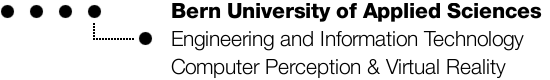
\includegraphics[width=46mm]{logo_ti.png}\newline

\emph{Module: Projektarbeit 2 (7302r)}\newline
\emph{Professor: Prof. Dr. Jürgen Eckerle}

\end{titlepage}


\tableofcontents


\newpage

\section{Disposition}

\subsection{Problem description}
Our task is to implement an event driven traffic simulation based upon a driver model, an environmental model and a vehicle model.


We have to provide models and simulate street traffic. 
The simulation is divided in three models:


\begin{enumerate}
 \item Environmental Model%Umgebungsmodell
 \item Driver Model%Fahrermodell
 \item Vehicle Model%Fahrzeugmodell
\end{enumerate}
The environmental and vehicle models have been mostly implemented already in our work in module 7301r. This project is based on that work.

\begin{center}
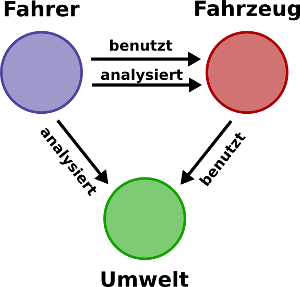
\includegraphics[width=5.5cm]{skizze.png}
\end{center}

\subsection{Objectives}
\subsubsection{Driver model}
 Create a parameterised driver model to be able to implement different 
 driver characters. These characters will be able to drive around autonomously 
 and make decisions based on the circumstances that they see and will be 
 influenced by parameters such as ``riskyness'' and temperament or drug intake.
 We are trying to achieve a high complexity in this field.

\subsubsection{Display}

Display the current state of the traffic situation. 
\newpage

\subsection{Optional Objectives}
\begin{enumerate}
 \item Changing the behaviour of the drivers by showing them road signs. 
 \item Obstruction of the view by buildings etc. 
\end{enumerate}
\subsection{Learning Goals}
Creation of an event driven simulation, applying basic principles of AI in the driver model.


\section{Organisation}

\subsection{Used Software}
\begin{tabular}{ll}
Programming Language & Java 6 \\
& \\
IDE & Eclipse \\
& \\
Documentation & \LaTeX \\
& \\
Version control & git \\
\end{tabular}

\subsection{Version control}
The version control is done with the free Tool Git\footnote[1]{http://git-scm.com}.
An online repository is hosted on github: \newline
http://github.com/schtibe/Projektarbeit-2-7302


\subsection{Involved Persons}

\begin{tabularx}{\textwidth}{XXX}
 Jürgen Eckerle & Professor & juergen.eckerle@bfh.ch \\
 Stefan Heinemann & Developer & heins4@bfh.ch \\
 Christoph Isch & Developer & ischc2@bfh.ch \\
\end{tabularx}

\subsection{Dates}

Start: 20.09.2010 \\
End: End of fall term 10/11

\section{System Requirements}

\subsection{Hardware}
\begin{enumerate}
 \item Intel Core 2 Duo
 \item 2 GB RAM
 \item GFX Card with 128 MB RAM
\end{enumerate}

Depending on the amount of simulated vehicles, the minimal requirements may not be sufficient.


\subsection{Software}
\begin{enumerate}
 \item Java Virtual Machine
\end{enumerate}


\section{Results}

The final results will be delivered in a zipped file.

\subsection{Application}
\begin{enumerate}
 \item Executable jar-file
 \item Sourcecode
\end{enumerate}

\subsection{Documentation}
\begin{enumerate}
 \item Project Specifications
 \item Javadoc
 \item Final Report
 \item Implementation
 \item Set up instructions
\end{enumerate}

All documents and all in-line documentation in code will be written in English.


\newpage
\begin{tabularx}{\textwidth}{XXX}
\textbf{Version} & \textbf{Date} & \textbf{Comment}\\
1 & 05.10.10 & \\
\end{tabularx}


\end{document}
